\section{Zielsetzung}
Ziel des Versuches war es, den Zusammenhang von Temperatur und Druck bei Wasser 
zu untersuchen. Dieser Zusammenhang lässt sich als Kurve festhalten,
einer Kurve, die diejenigen Temperaturen und Drücke enthält, bei denen im Wasser
ein Phasenübergang stattfinden würde, also ein Übergang von einem Aggregatzustand
in einen anderen. So gibt es in dem Diagramm drei Gebiete, wie sie in Abbildung \ref{fig:kurve}
\begin{figure}
    \centering
    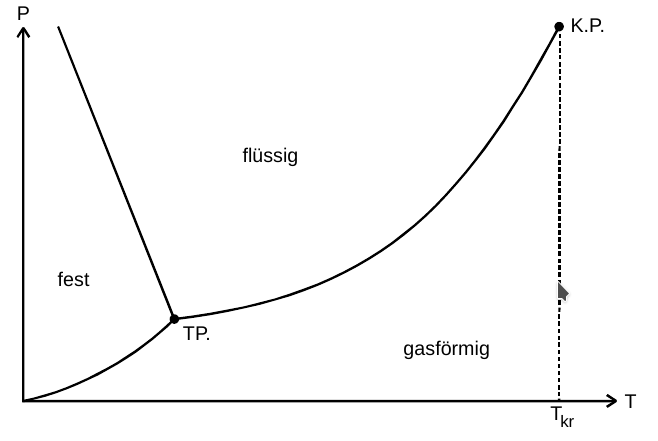
\includegraphics[width=\textwidth]{dampfdruckkurve.png}
    \caption{Qualitative Darstellung der Dampfdruckkurve für Wasser.(Quelle [1])}
    \label{fig:kurve}
\end{figure}
zu sehen sind. \\